Aqu\'i se describir\'an los objetivos que tiene el equipo de desarrollo, as\'i como la arquitectura que tendr\'a el sistema, y la especificaci\'on t\'ecnica que tiene la plataforma sobre la que ser\'a instalado el sistema, tanto de software como de hardware.

%--------------------------------------------------
\section{Objetivos}

% - - - - - - - - - - - - - - - - - - - - - - - - -
\subsection{Objetivo general}
Crear un sistema en el que puedan solucionar todas las problem\'aticas descritas anteriormente de la cl\'inica m\'edica, de forma eficaz y eficiente.


% - - - - - - - - - - - - - - - - - - - - - - - - -
\subsection{Objetivos específicos}


\begin{itemize}
\item Llevar a cabo el proceso de citas por internet, donde el paciente podr\'a seleccionar la hora y fecha en la que solicitar\'a una cita m\'edica.
\item Usar un repositorio de datos electr\'onico para contener los expedientes m\'edicos de los pacientes de la cl\'inica.
\item Tener control e informar sobre el stock del almac\'en en la farmacia.
\item Poder informar al cliente si la cita puede realizarse en la fecha y hora dados, con base a la disponibilidad de consultorios. En
caso de que est\'en agotada en un horario y fecha determinados, el paciente podr\'a volver a solicitar una cita.
\item Definir una forma para gestionar los expedientes m\'edicos.
\item Tener una forma m\'as segura para almacenar la inform\'aci\'on (expedientes m\'edicos, transacciones, dinero de la caja, citas m\'edicas y stock de medicamentos en almac\'en.
\item Generar recetas de forma m\'as r\'apida y f\'acil para el m\'edico.

\end{itemize}
\hspace{-.50cm}
\hspace{-.50cm}


% - - - - - - - - - - - - - - - - - - - - - - - - -
\subsection{Requerimientos no funcionales}

\begin{figure}[htbp!]
		\centering		
	\end{figure}

\begin{table}[h]
\hspace{-.50cm}
\begin{tabular}{|l|l|l|}
\hline
	\multicolumn{1}{|c|}{\textbf{ID}} & \multicolumn{1}{c|}{\textbf{Nombre}} & \multicolumn{1}{c|}{\textbf{Descripci\'on}} \\ \hline
	RNF1 & Forma de almacenamiento & \begin{tabular}[c]{@{}l@{}}La informaci\'on requerida se guardar\'a en una base de datos de MySQL
																														 \end{tabular} \\ \hline
	RNF2	& Cupo de horario & \begin{tabular}[c]{@{}l@{}}Mediante consultas de SQL, la plataforma web determinar\'a si es posible realizar\\una cita en el horario seleccionado
																											 \end{tabular} \\ \hline
	RNF3 & Tecnolog\'ias web & \begin{tabular}[c]{@{}l@{}}Para la plataforma web se usar\'an las tecnolog\'ias HTML, CSS y PHP
																													 \end{tabular} \\ \hline
	RNF4 & \begin{tabular}[c]{@{}l@{}}Selecci\'on de horario \end{tabular} & 
	\begin{tabular}[c]{@{}l@{}}El sistema le mostrar\'a al usuario los horarios disponibles \\ en intervalos de media hora. \end{tabular} \\ \hline
																															
\end{tabular}
\caption{Requerimientos no funcionales}
\end{table}


% - - - - - - - - - - - - - - - - - - - - - - - - -
\subsection{Modelo de despliegue del sistema}


	\begin{figure}[htbp!]
		\centering
			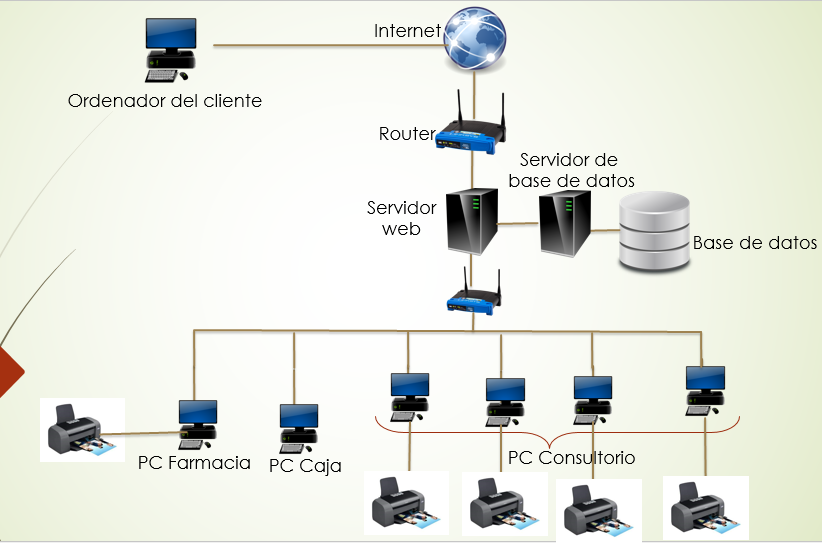
\includegraphics[width=1.15\textwidth]{images/mod_fis3.png}
		\caption{Diagrama de arquitectura.}
	\end{figure}



% - - - - - - - - - - - - - - - - - - - - - - - - -
\subsection{Especificación de Plataforma}
Caracter\'isticas que cuentan los equipos sobre los cu\'ales se implement\'o o us\'o la plataforma (servidor y cliente, respectivamente):


\bfseries Servidor (Hardware): \mdseries
\begin{itemize}
\item Procesador AMD A10-4600M APU
\item 6 GB RAM DDR3
\item Motherboard InsydeH2O CCB.03.72.306.00
\end{itemize}

\bfseries Servidor (Software): \mdseries
\begin{itemize}
\item Windows 8 x64 (6.2, compilaci\'on 9200)
\item Apache 2.4.20
\item MySQL 5.7.12
\end{itemize}

\bfseries Cliente-clinica (Hardware): \mdseries
\begin{itemize}
\item Procesador AMD A10-4600M APU
\item 6 GB RAM DDR3
\item Motherboard InsydeH2O CCB.03.72.306.00
\end{itemize}

\bfseries Cliente-clinica (Software): \mdseries
\begin{itemize}
\item Windows 8 x64 (6.2, compilaci\'on 9200)
\item MySQL 5.7.12
\item Java Version 8 Update 91
\end{itemize}

